\documentclass[review]{elsarticle}
\usepackage{graphicx}
\usepackage{hyperref}

%% To allow supplementary table and figure numbering
%% http://bytesizebio.net/2013/03/11/adding-supplementary-tables-and-figures-in-latex/

\newcommand{\beginsupplement}{%
		        \setcounter{table}{0}
		        \renewcommand{\thetable}{S\arabic{table}}%
		        \setcounter{figure}{0}
		        \renewcommand{\thefigure}{S\arabic{figure}}%
			     }

\journal{Ecological Modelling}

\title{MixFishSim: Supplementary Figures and Tables}

\begin{document}

\beginsupplement
\maketitle

\begin{figure}[!ht]
	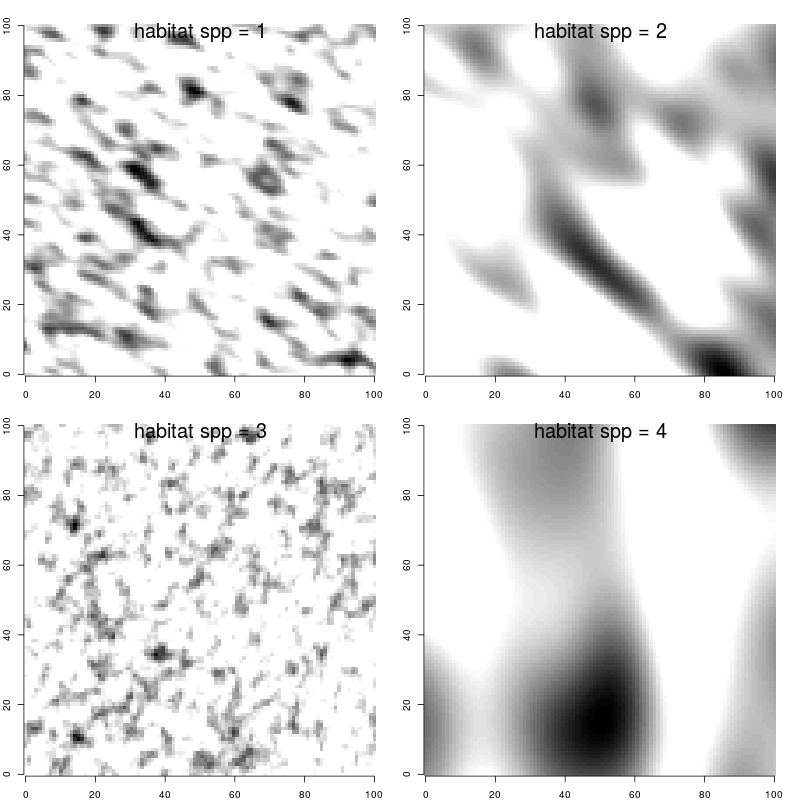
\includegraphics[width = \linewidth]{../tests/plots/habitat}
	\caption{habitat preference}
	\label{fig:1}
\end{figure}	

\begin{figure}[!ht]
	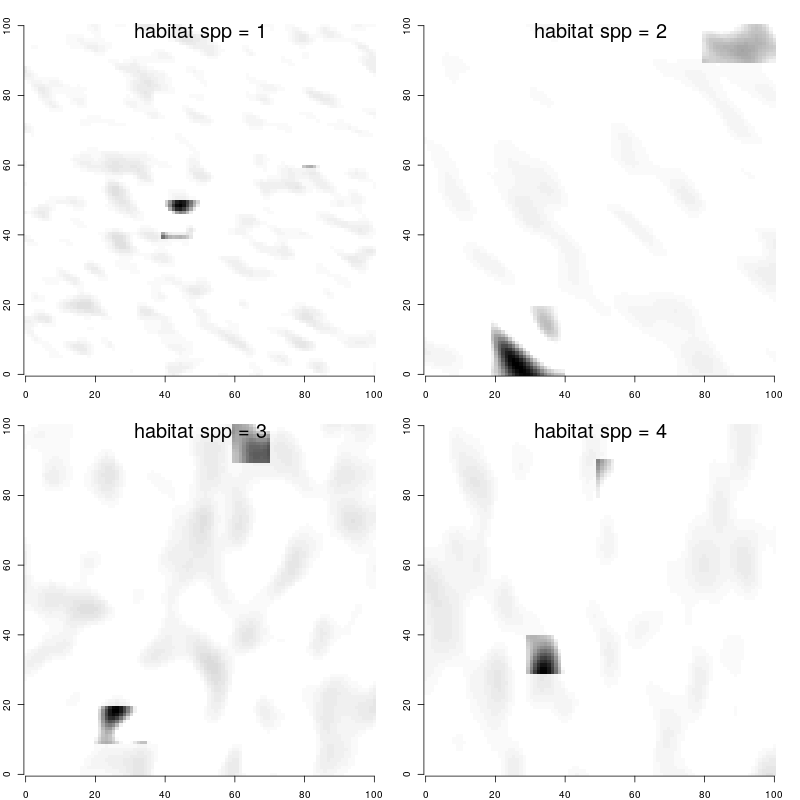
\includegraphics[width = \linewidth]{Plots/habitat_spwn}
	\caption{spawning habitat preference}
	\label{fig:2}
\end{figure}	


\begin{figure}[!ht]
	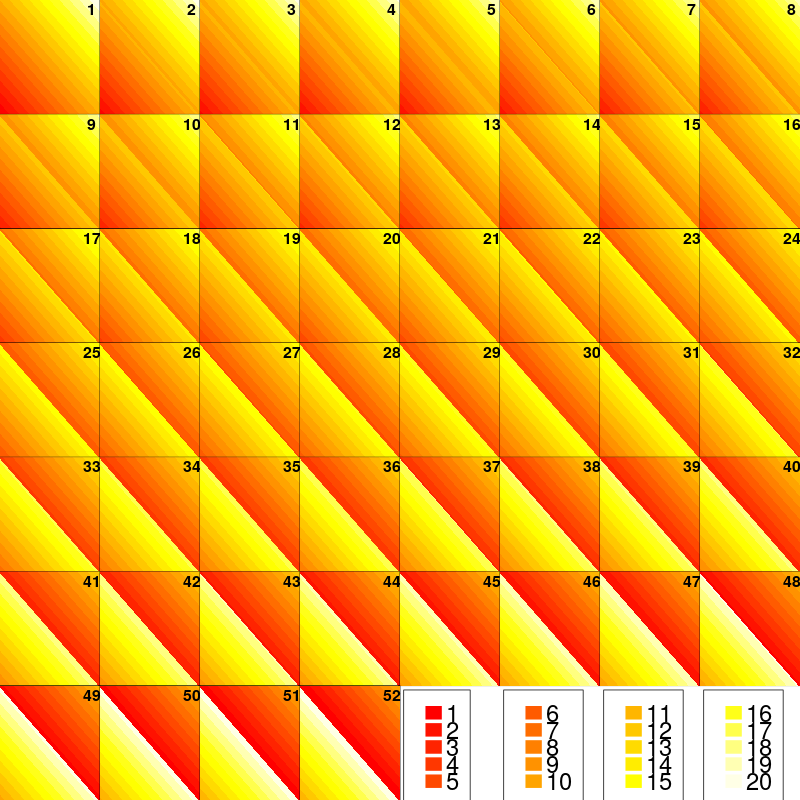
\includegraphics[width = \linewidth]{Plots/Temperature_gradient}
	\caption{Spatiotemporal qemperature gradient}
	\label{fig:3}
\end{figure}

\begin{figure}[!ht]
	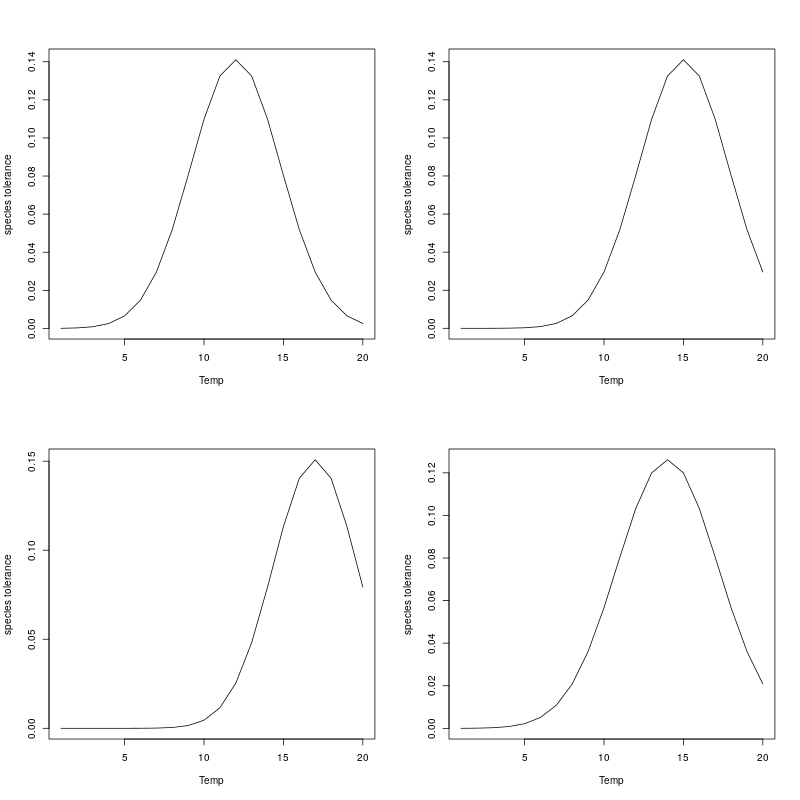
\includegraphics[width = \linewidth]{Plots/Species_tolerances}
	\caption{Species thermal tolerances}
	\label{fig:4}
\end{figure}

\begin{figure}[!ht]
	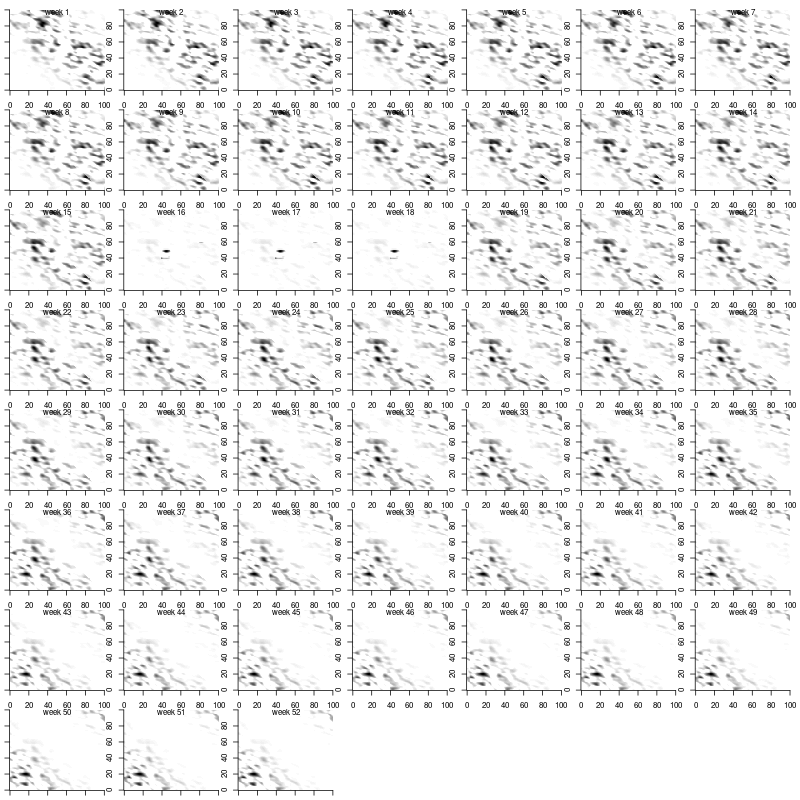
\includegraphics[width = \linewidth]{Plots/habitat_spatiotemp_spp_1}
	\caption{Spatiotemporal habitat suitability - population 1}
	\label{fig:5}
\end{figure}

\begin{figure}[!ht]
	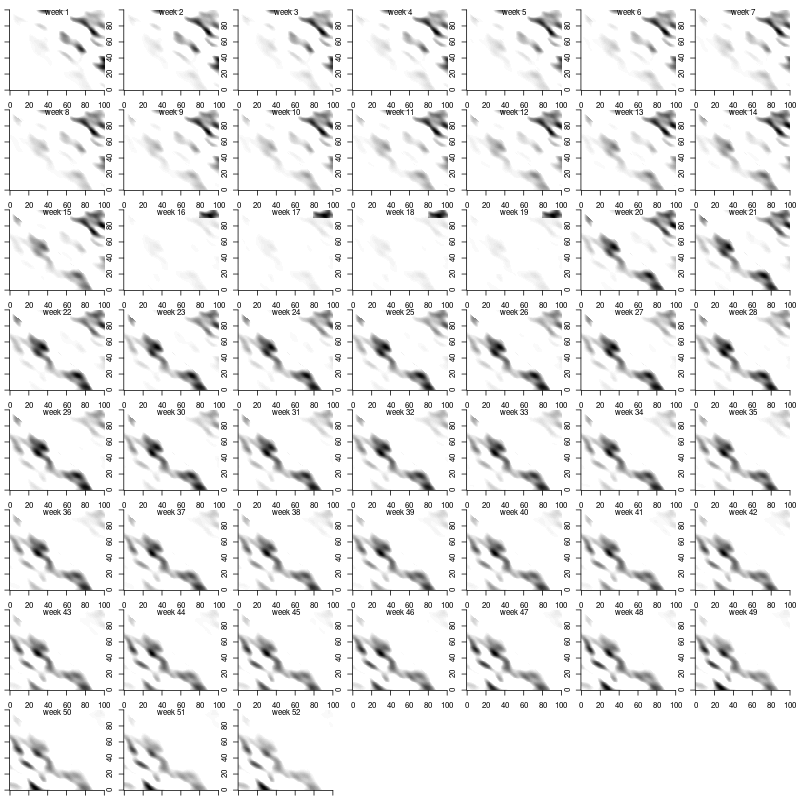
\includegraphics[width = \linewidth]{Plots/habitat_spatiotemp_spp_2}
	\caption{Spatiotemporal habitat suitability - population 2}
	\label{fig:6}
\end{figure}

\begin{figure}[!ht]
	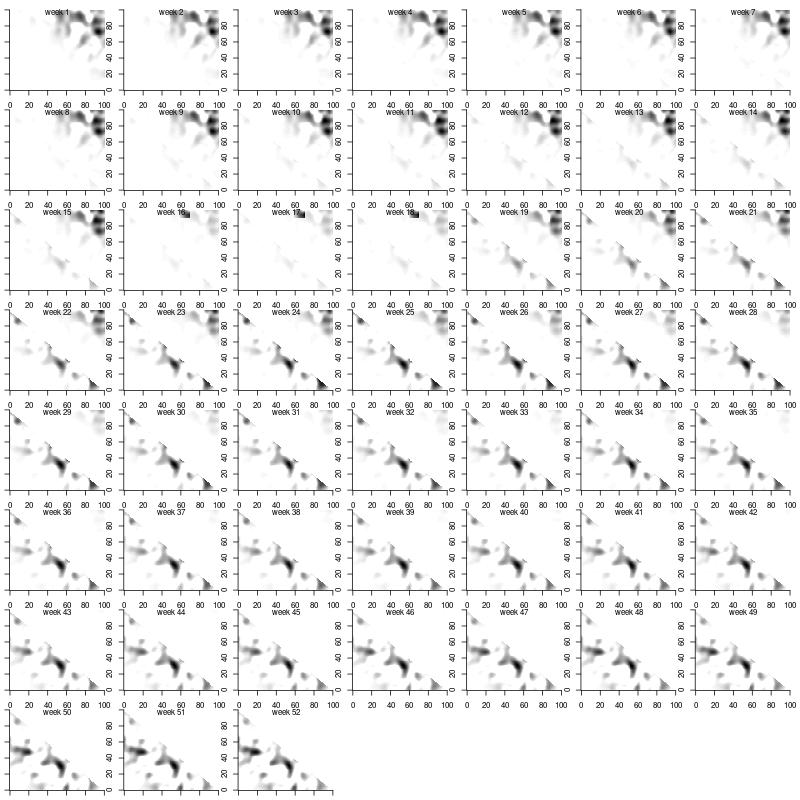
\includegraphics[width = \linewidth]{Plots/habitat_spatiotemp_spp_3}
	\caption{Spatiotemporal habitat suitability - population 3}
	\label{fig:7}
\end{figure}

\begin{figure}[!ht]
	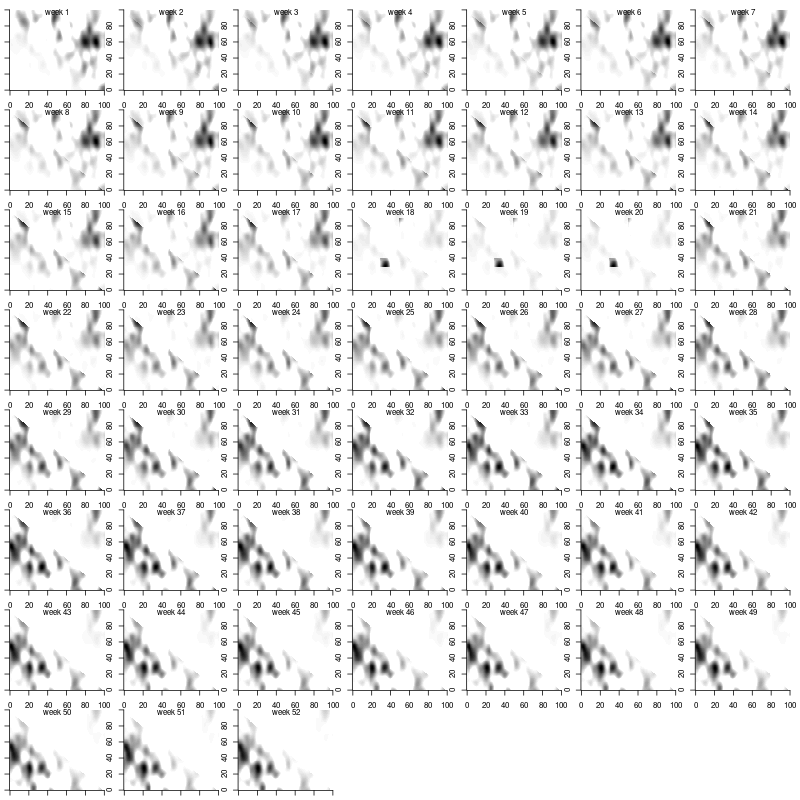
\includegraphics[width = \linewidth]{Plots/habitat_spatiotemp_spp_4}
	\caption{Spatiotemporal habitat suitability - population 4}
	\label{fig:8}
\end{figure}



\begin{figure}[!ht]
	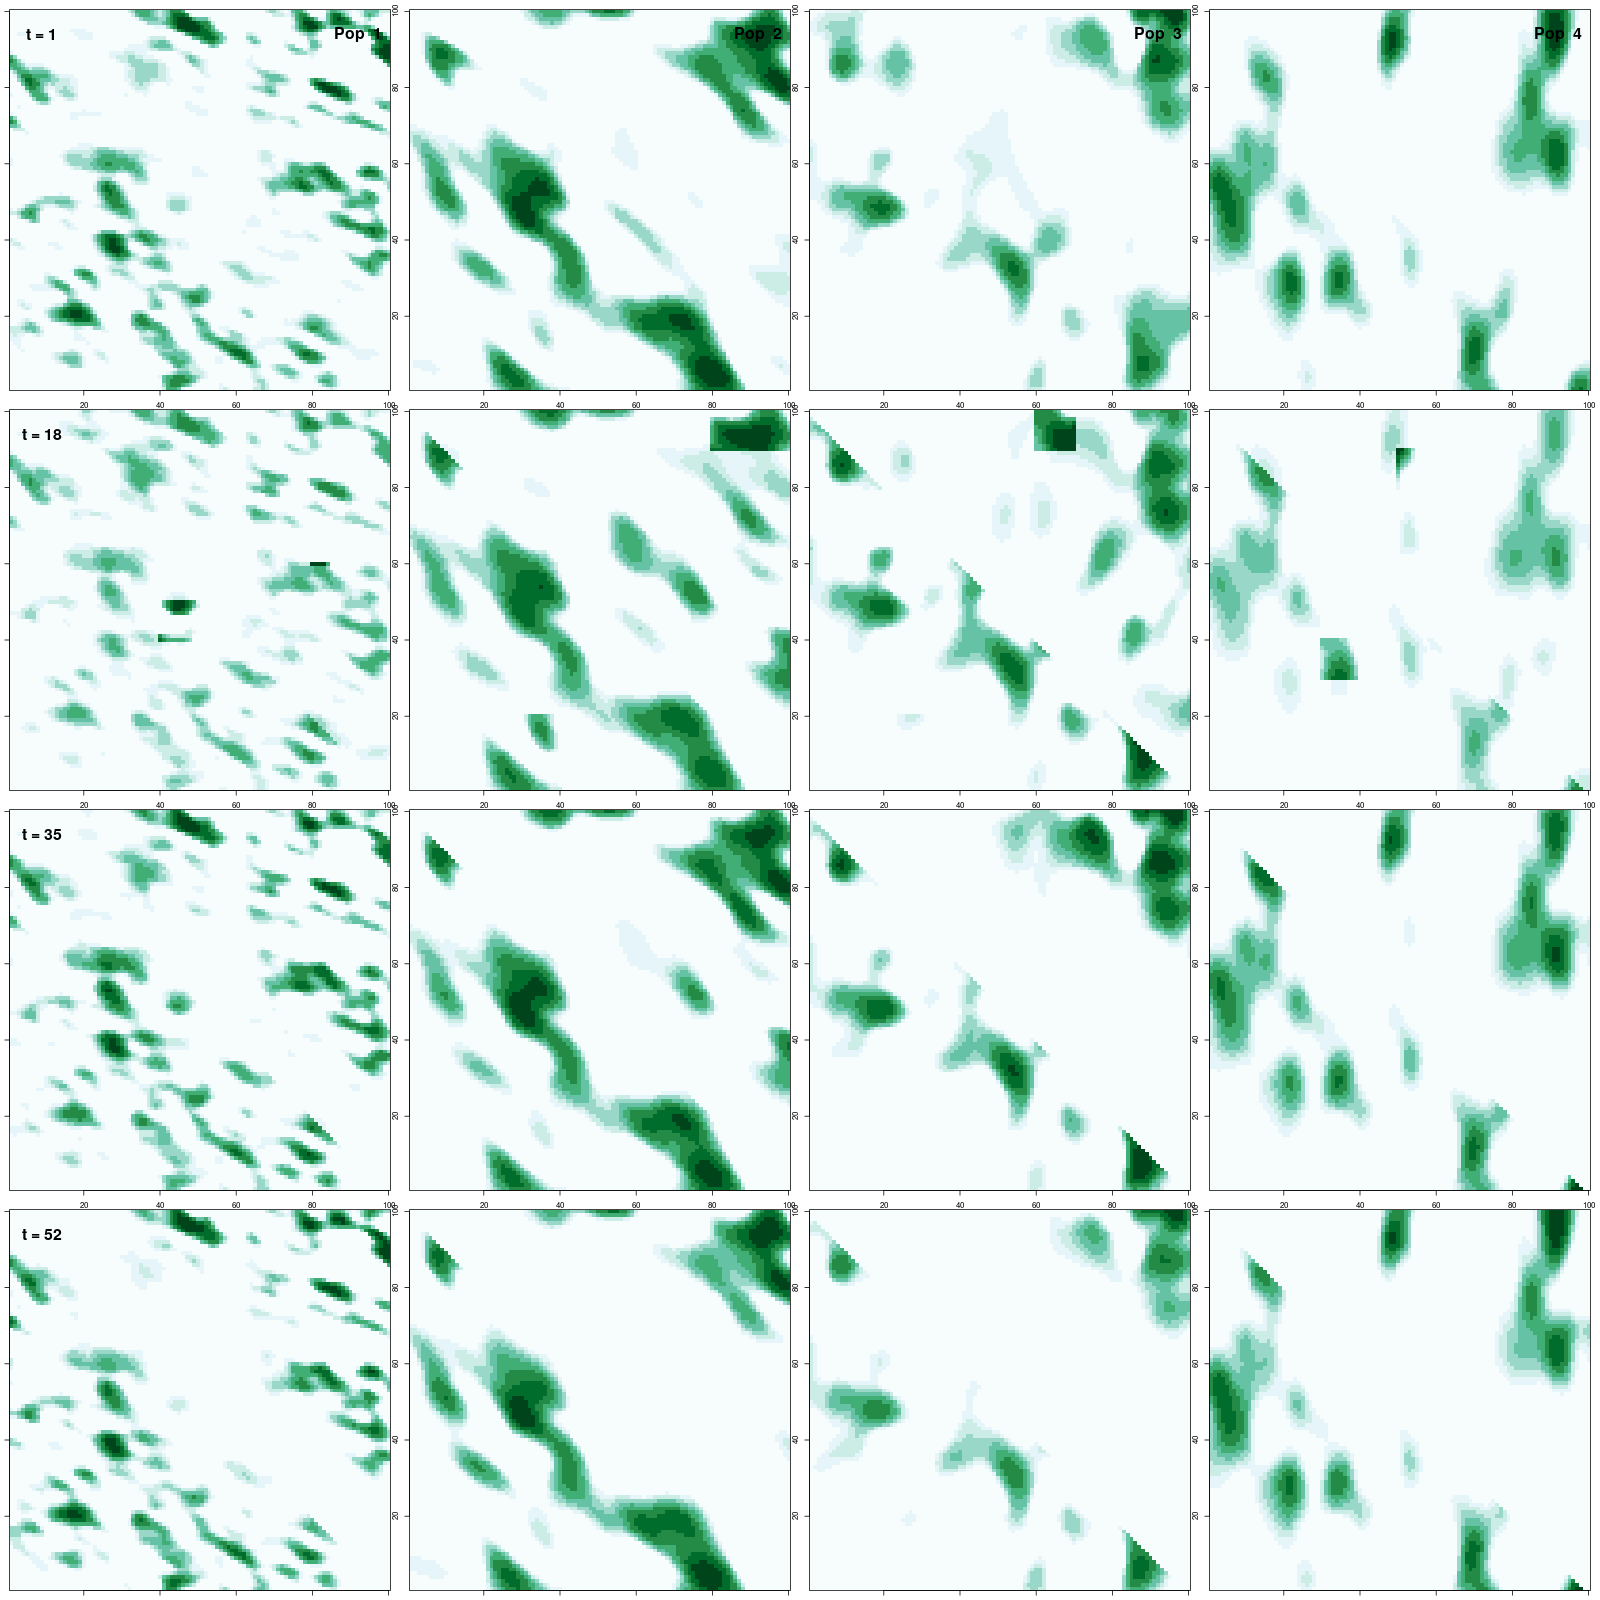
\includegraphics[width = \linewidth]{Plots/pop_dist}
	\caption{Simulated spatial dynamics - the four populations at four time steps.
		}
	\label{fig:9}
\end{figure}	

\begin{figure}[!ht]
	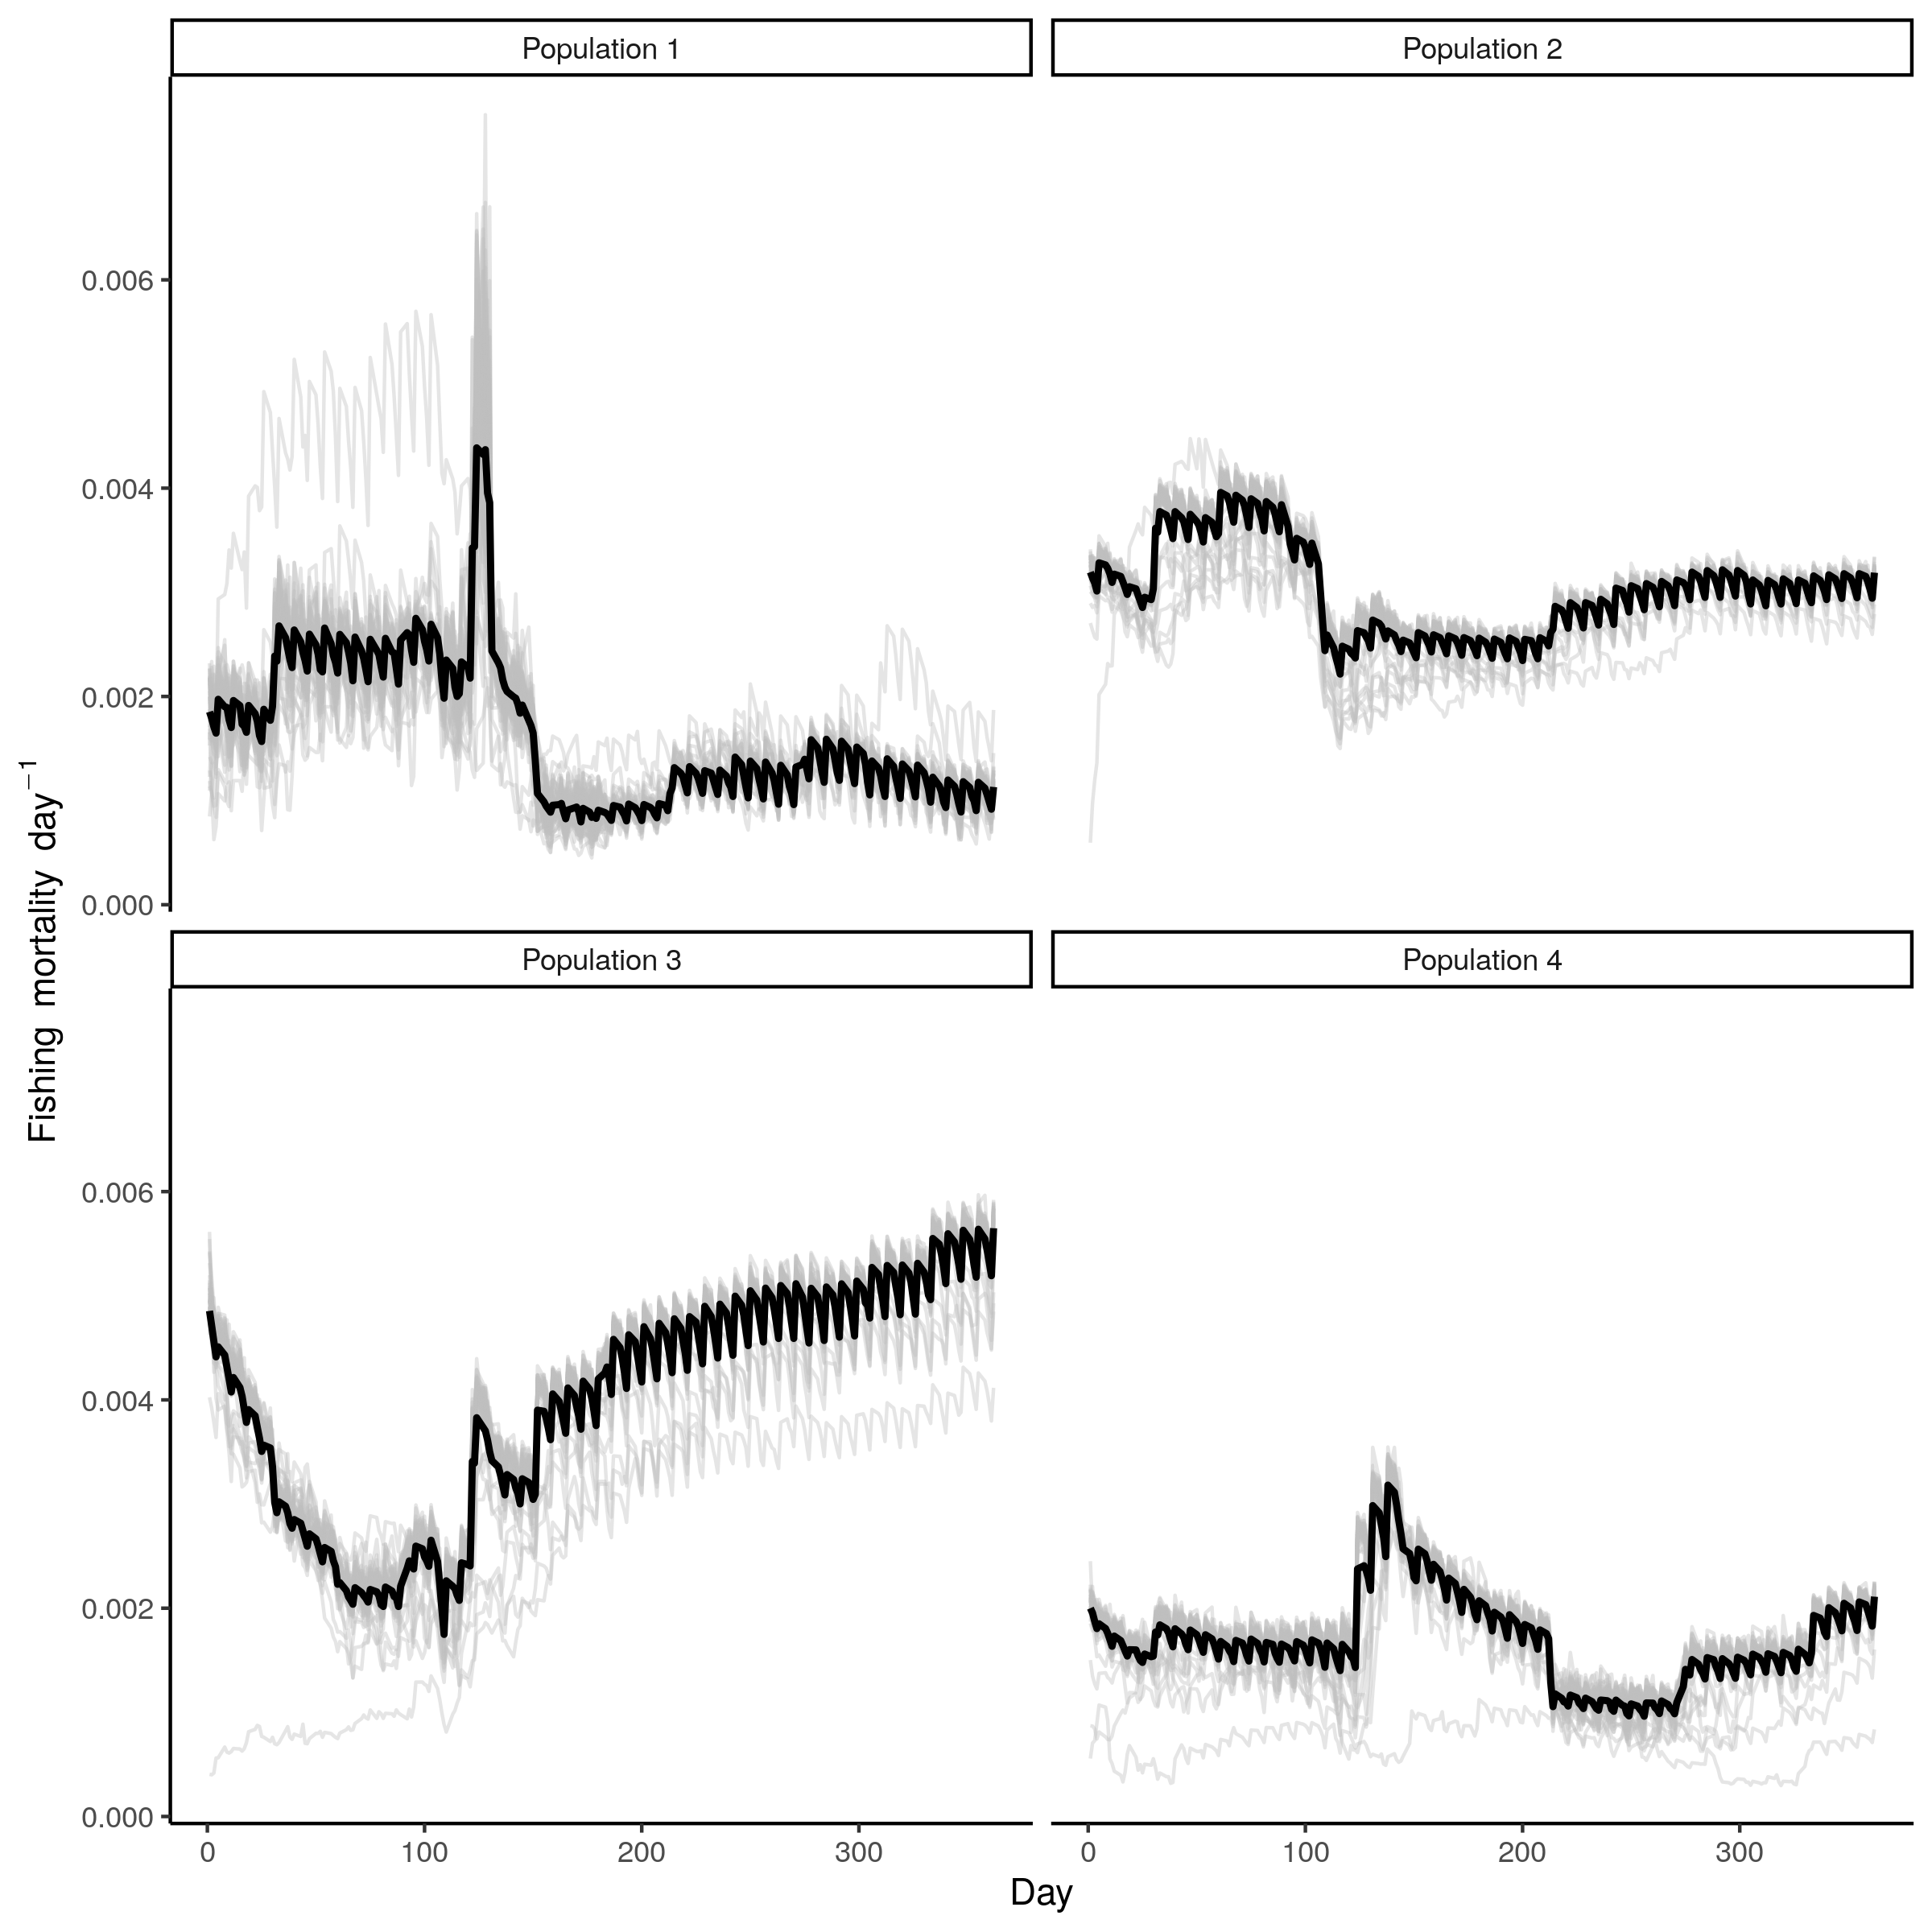
\includegraphics[width = \linewidth]{Plots/f_dynamics}
	\caption{f dynamics - the daily fishing mortalities, each year is a
		different colour}
	\label{fig:10}
\end{figure}	

\begin{figure}[!ht]
	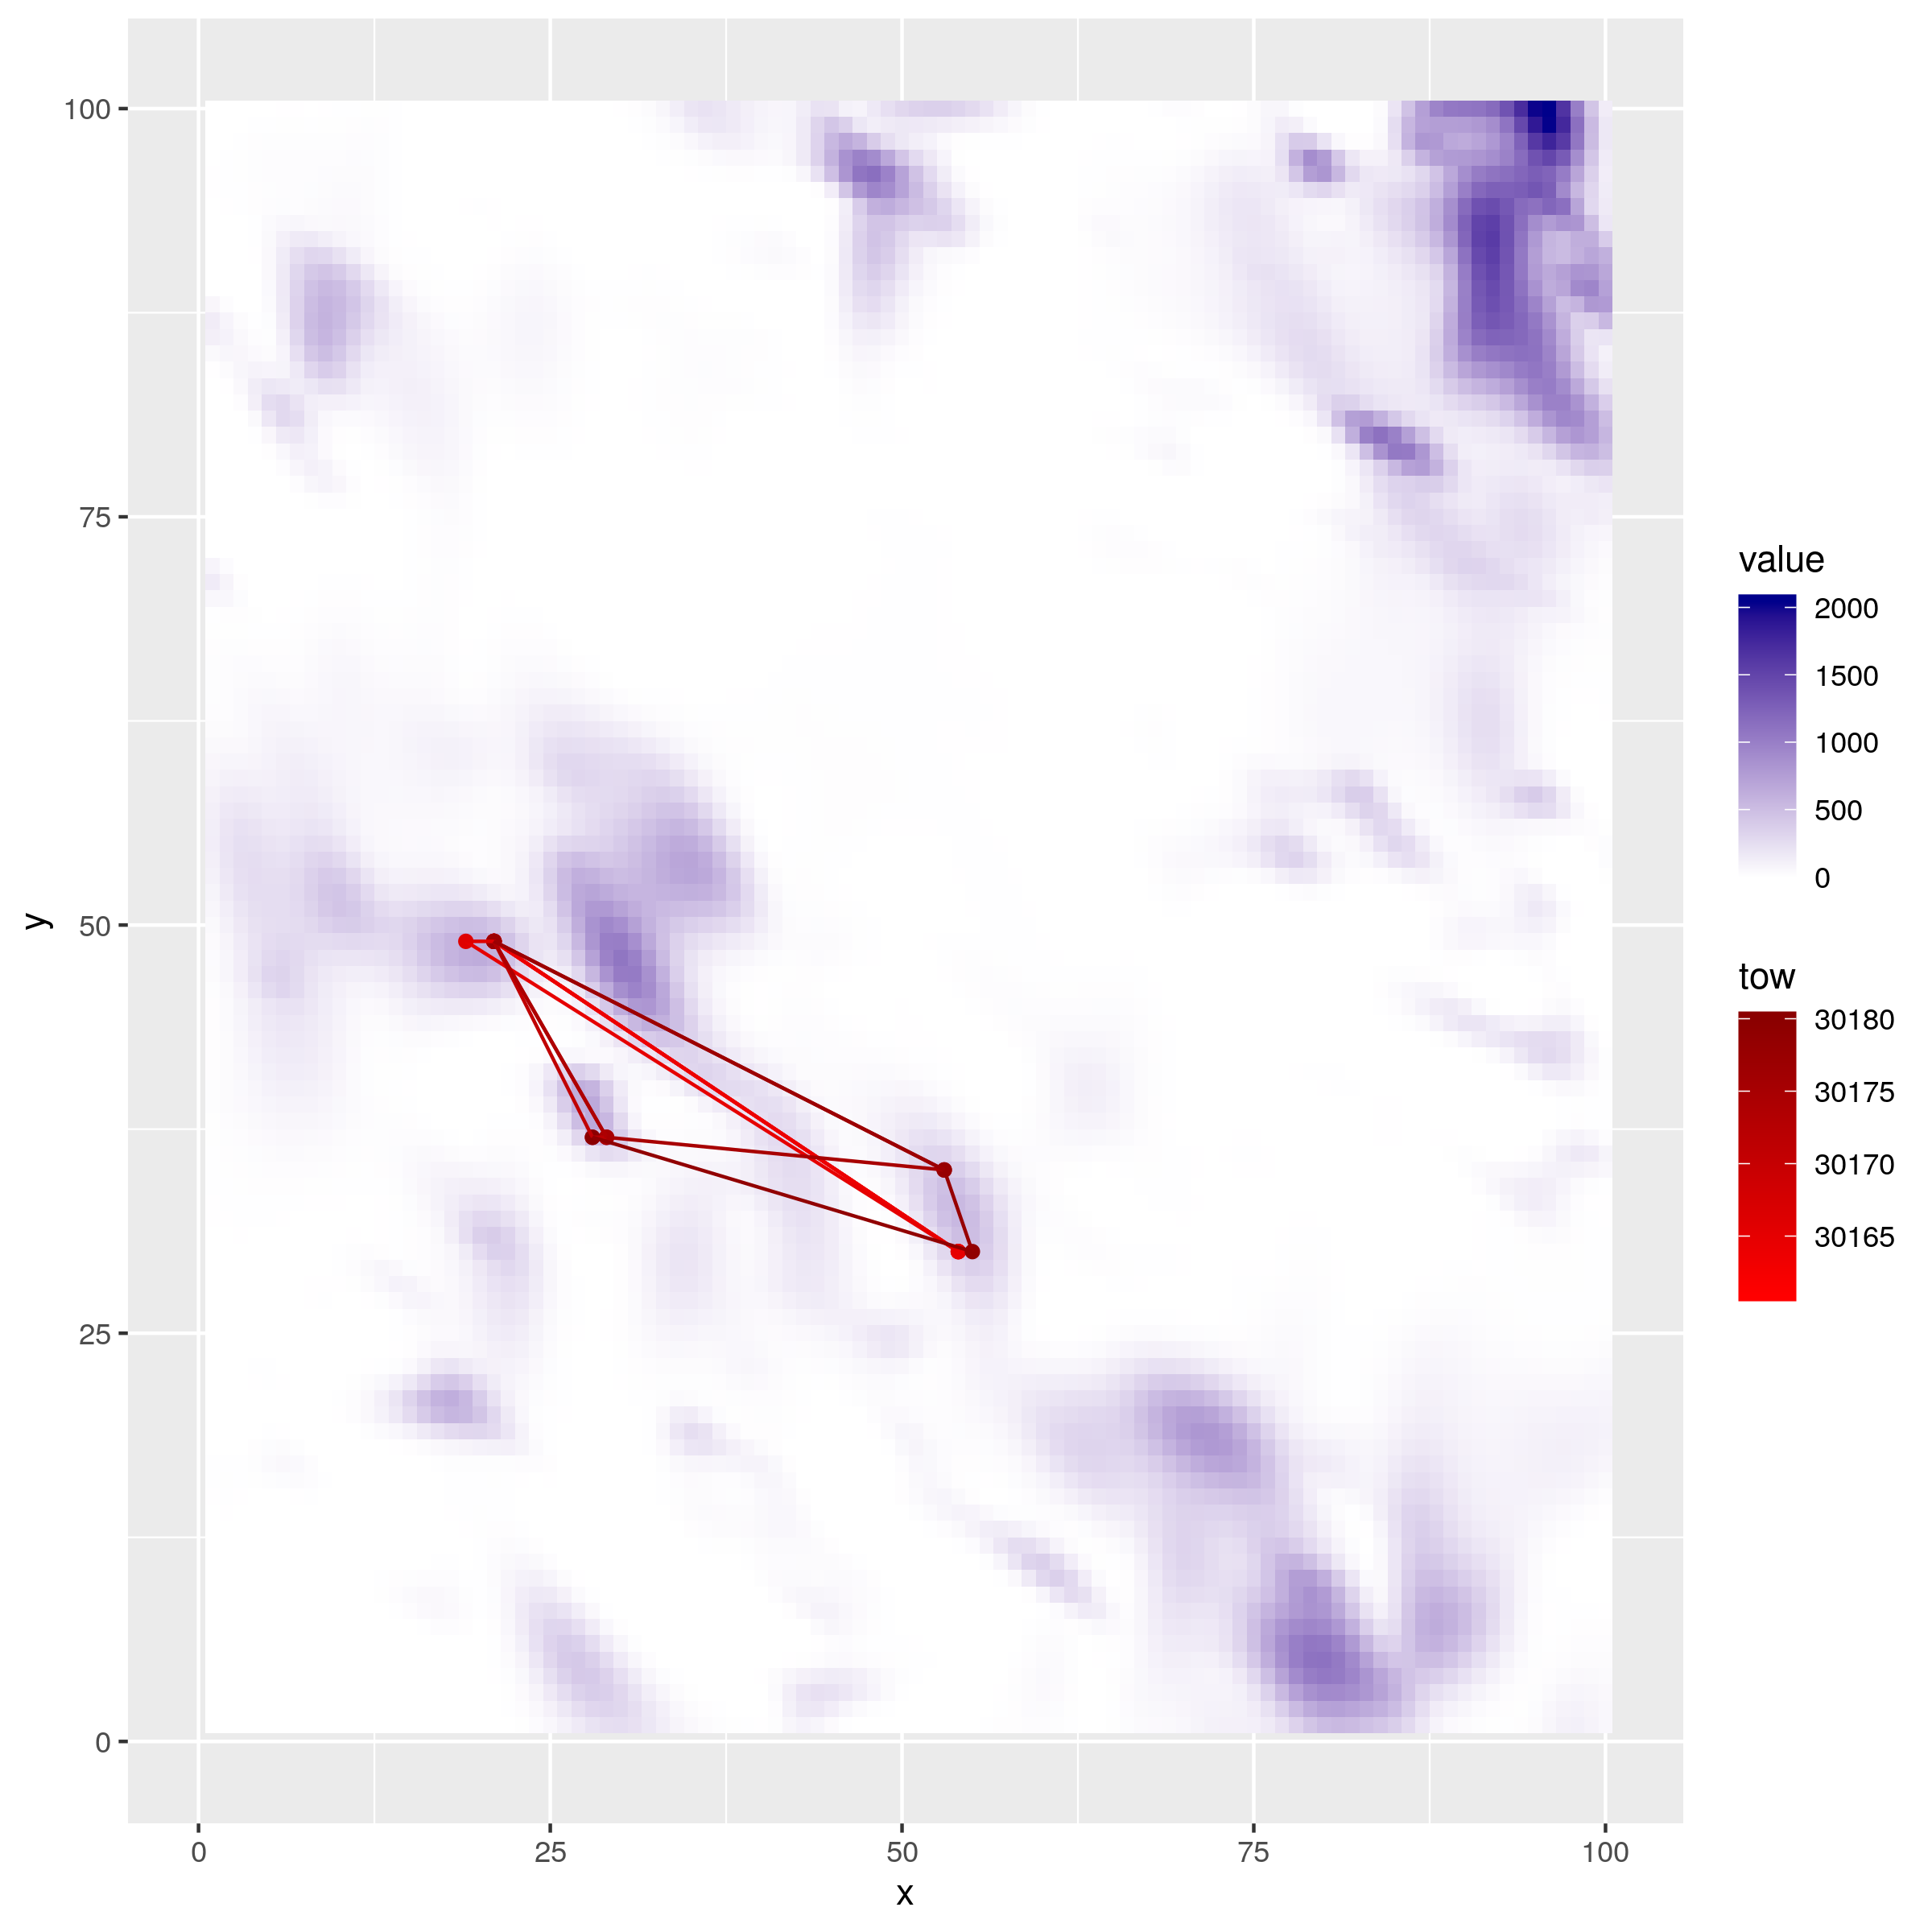
\includegraphics[width = \linewidth]{Plots/vessel_move}
	\caption{vessel movement - a single trip movement for one vessel}
	\label{fig:11}
\end{figure}	

\begin{figure}[!ht]
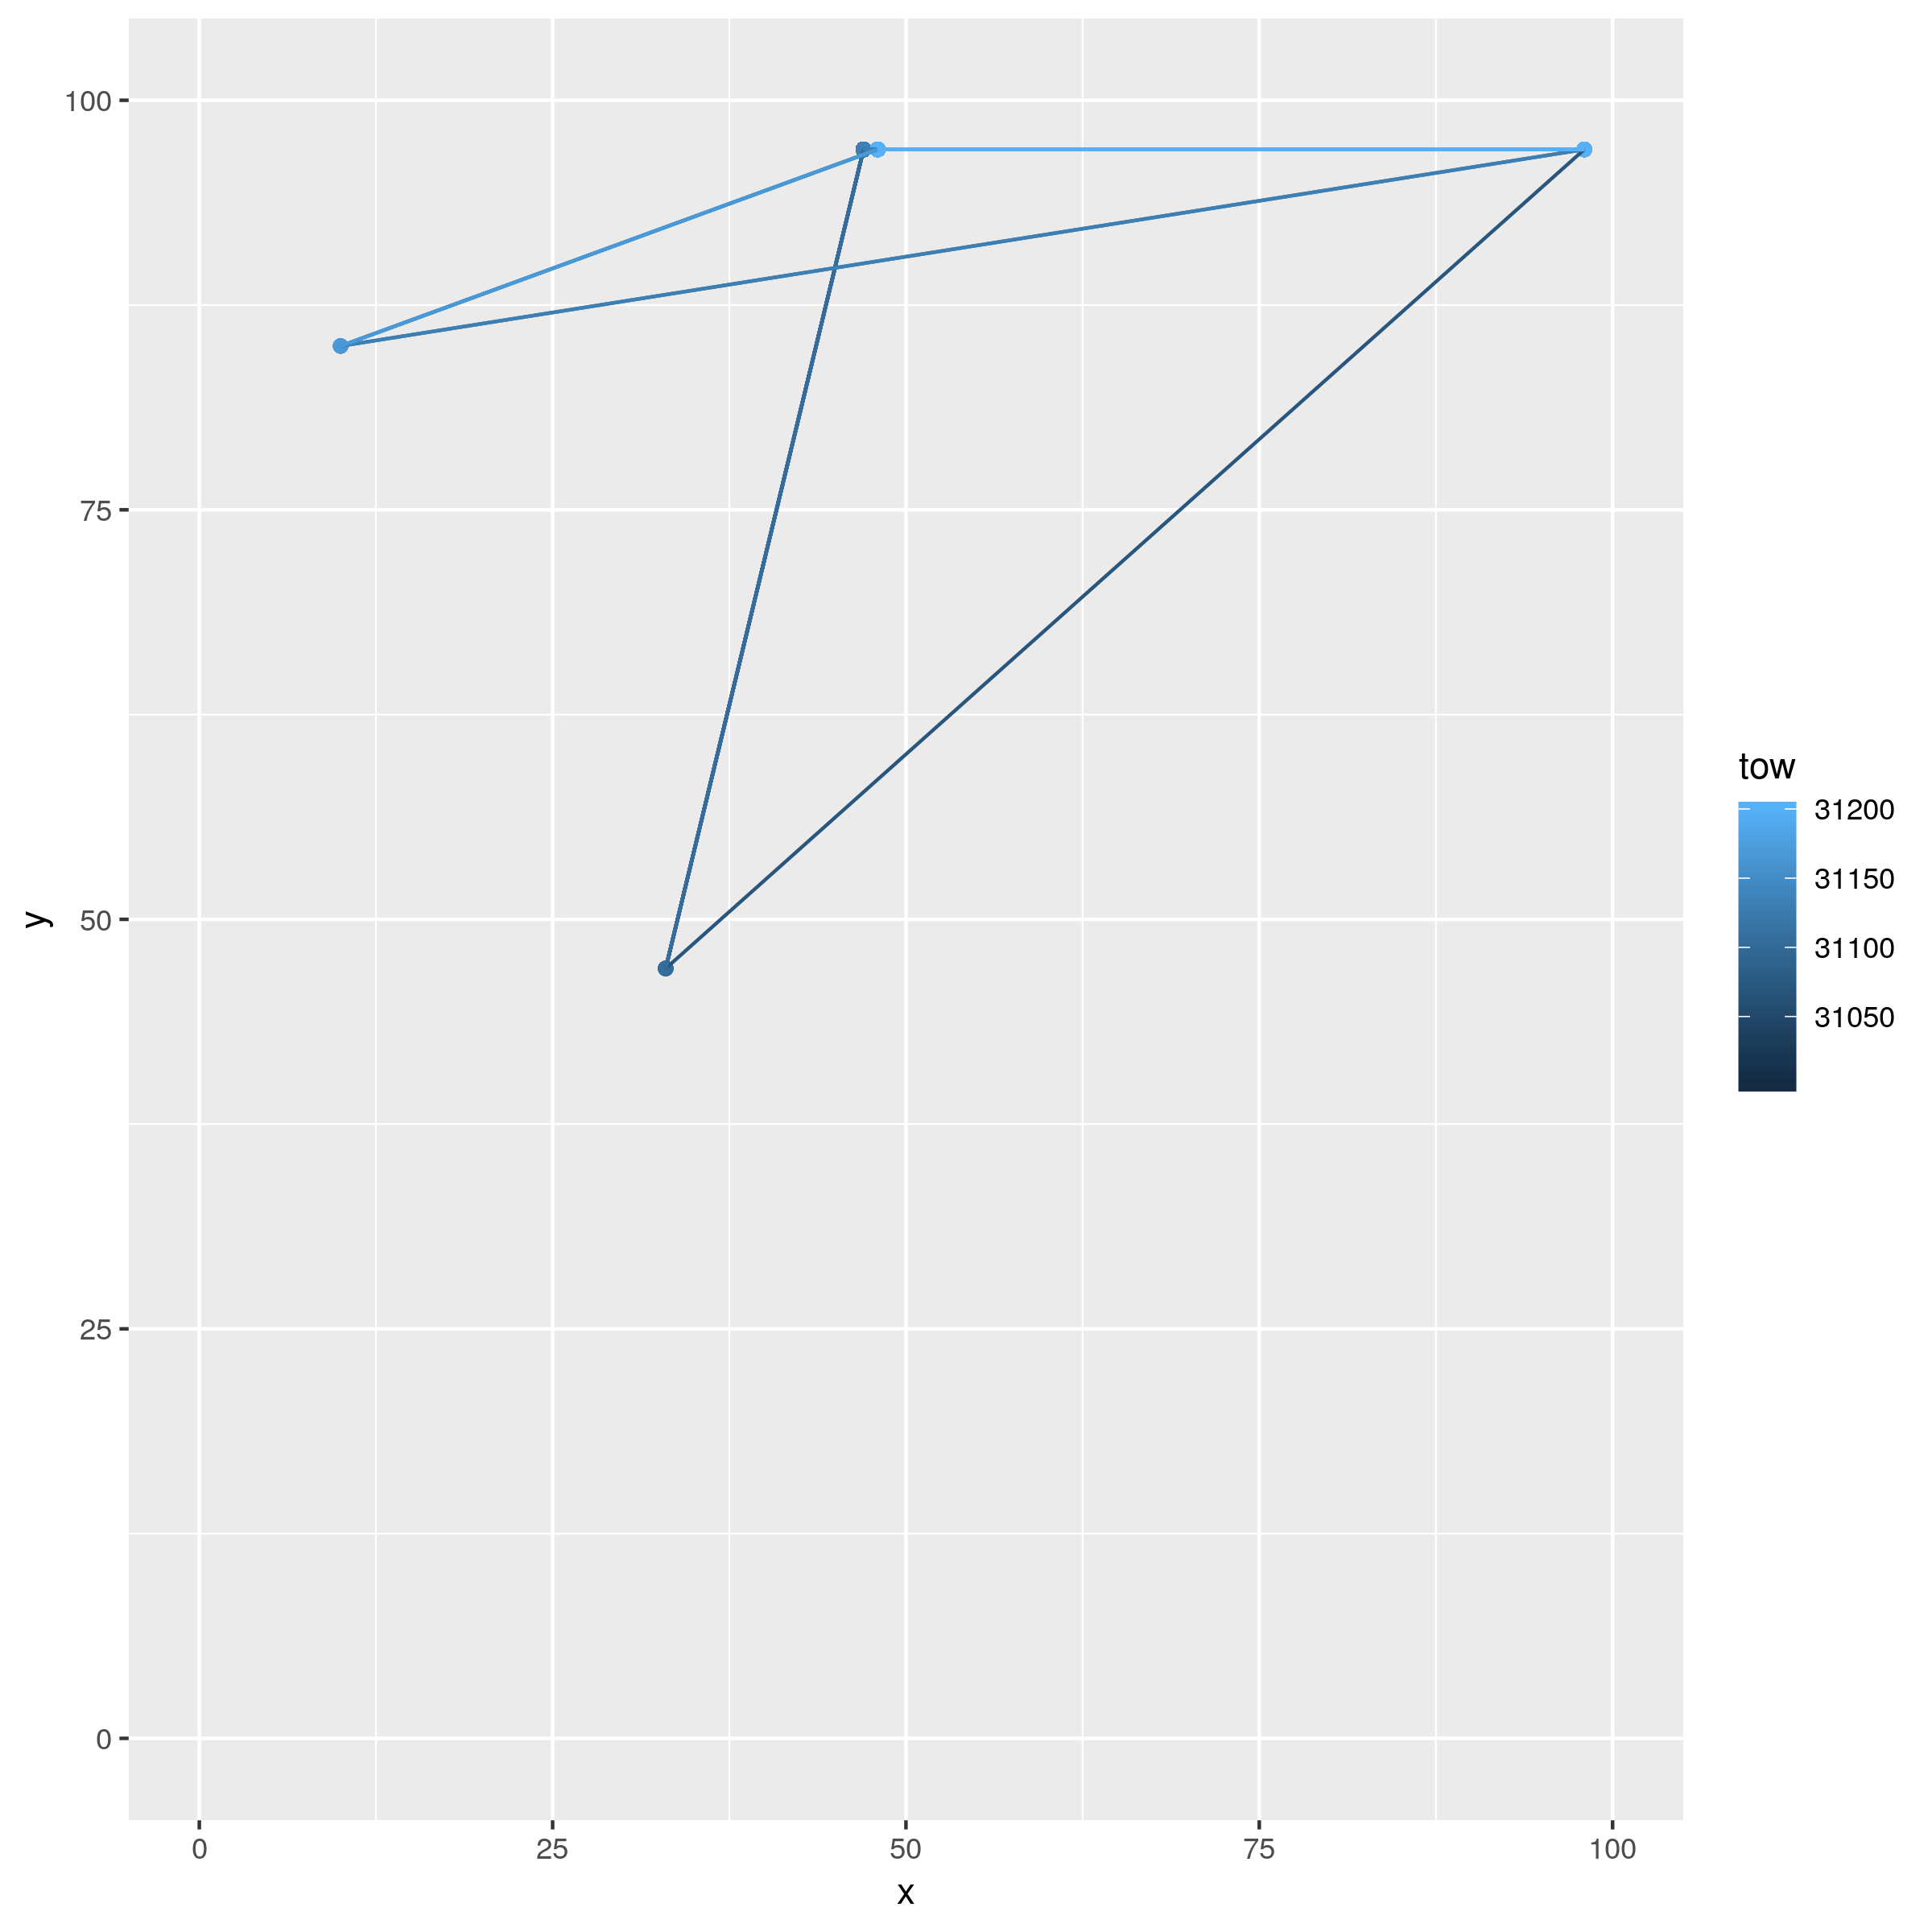
\includegraphics[width = \linewidth]{Plots/vessel_multi_move}
	\caption{vessel movement for multiple trips from a single vessel. Note
	the movement off the side pops up the other side, but is joined by a
	line across the grid. This is from the torus approach rather than the
	edges being barriers}
	\label{fig:12}
\end{figure}	

\begin{figure}[!ht]
	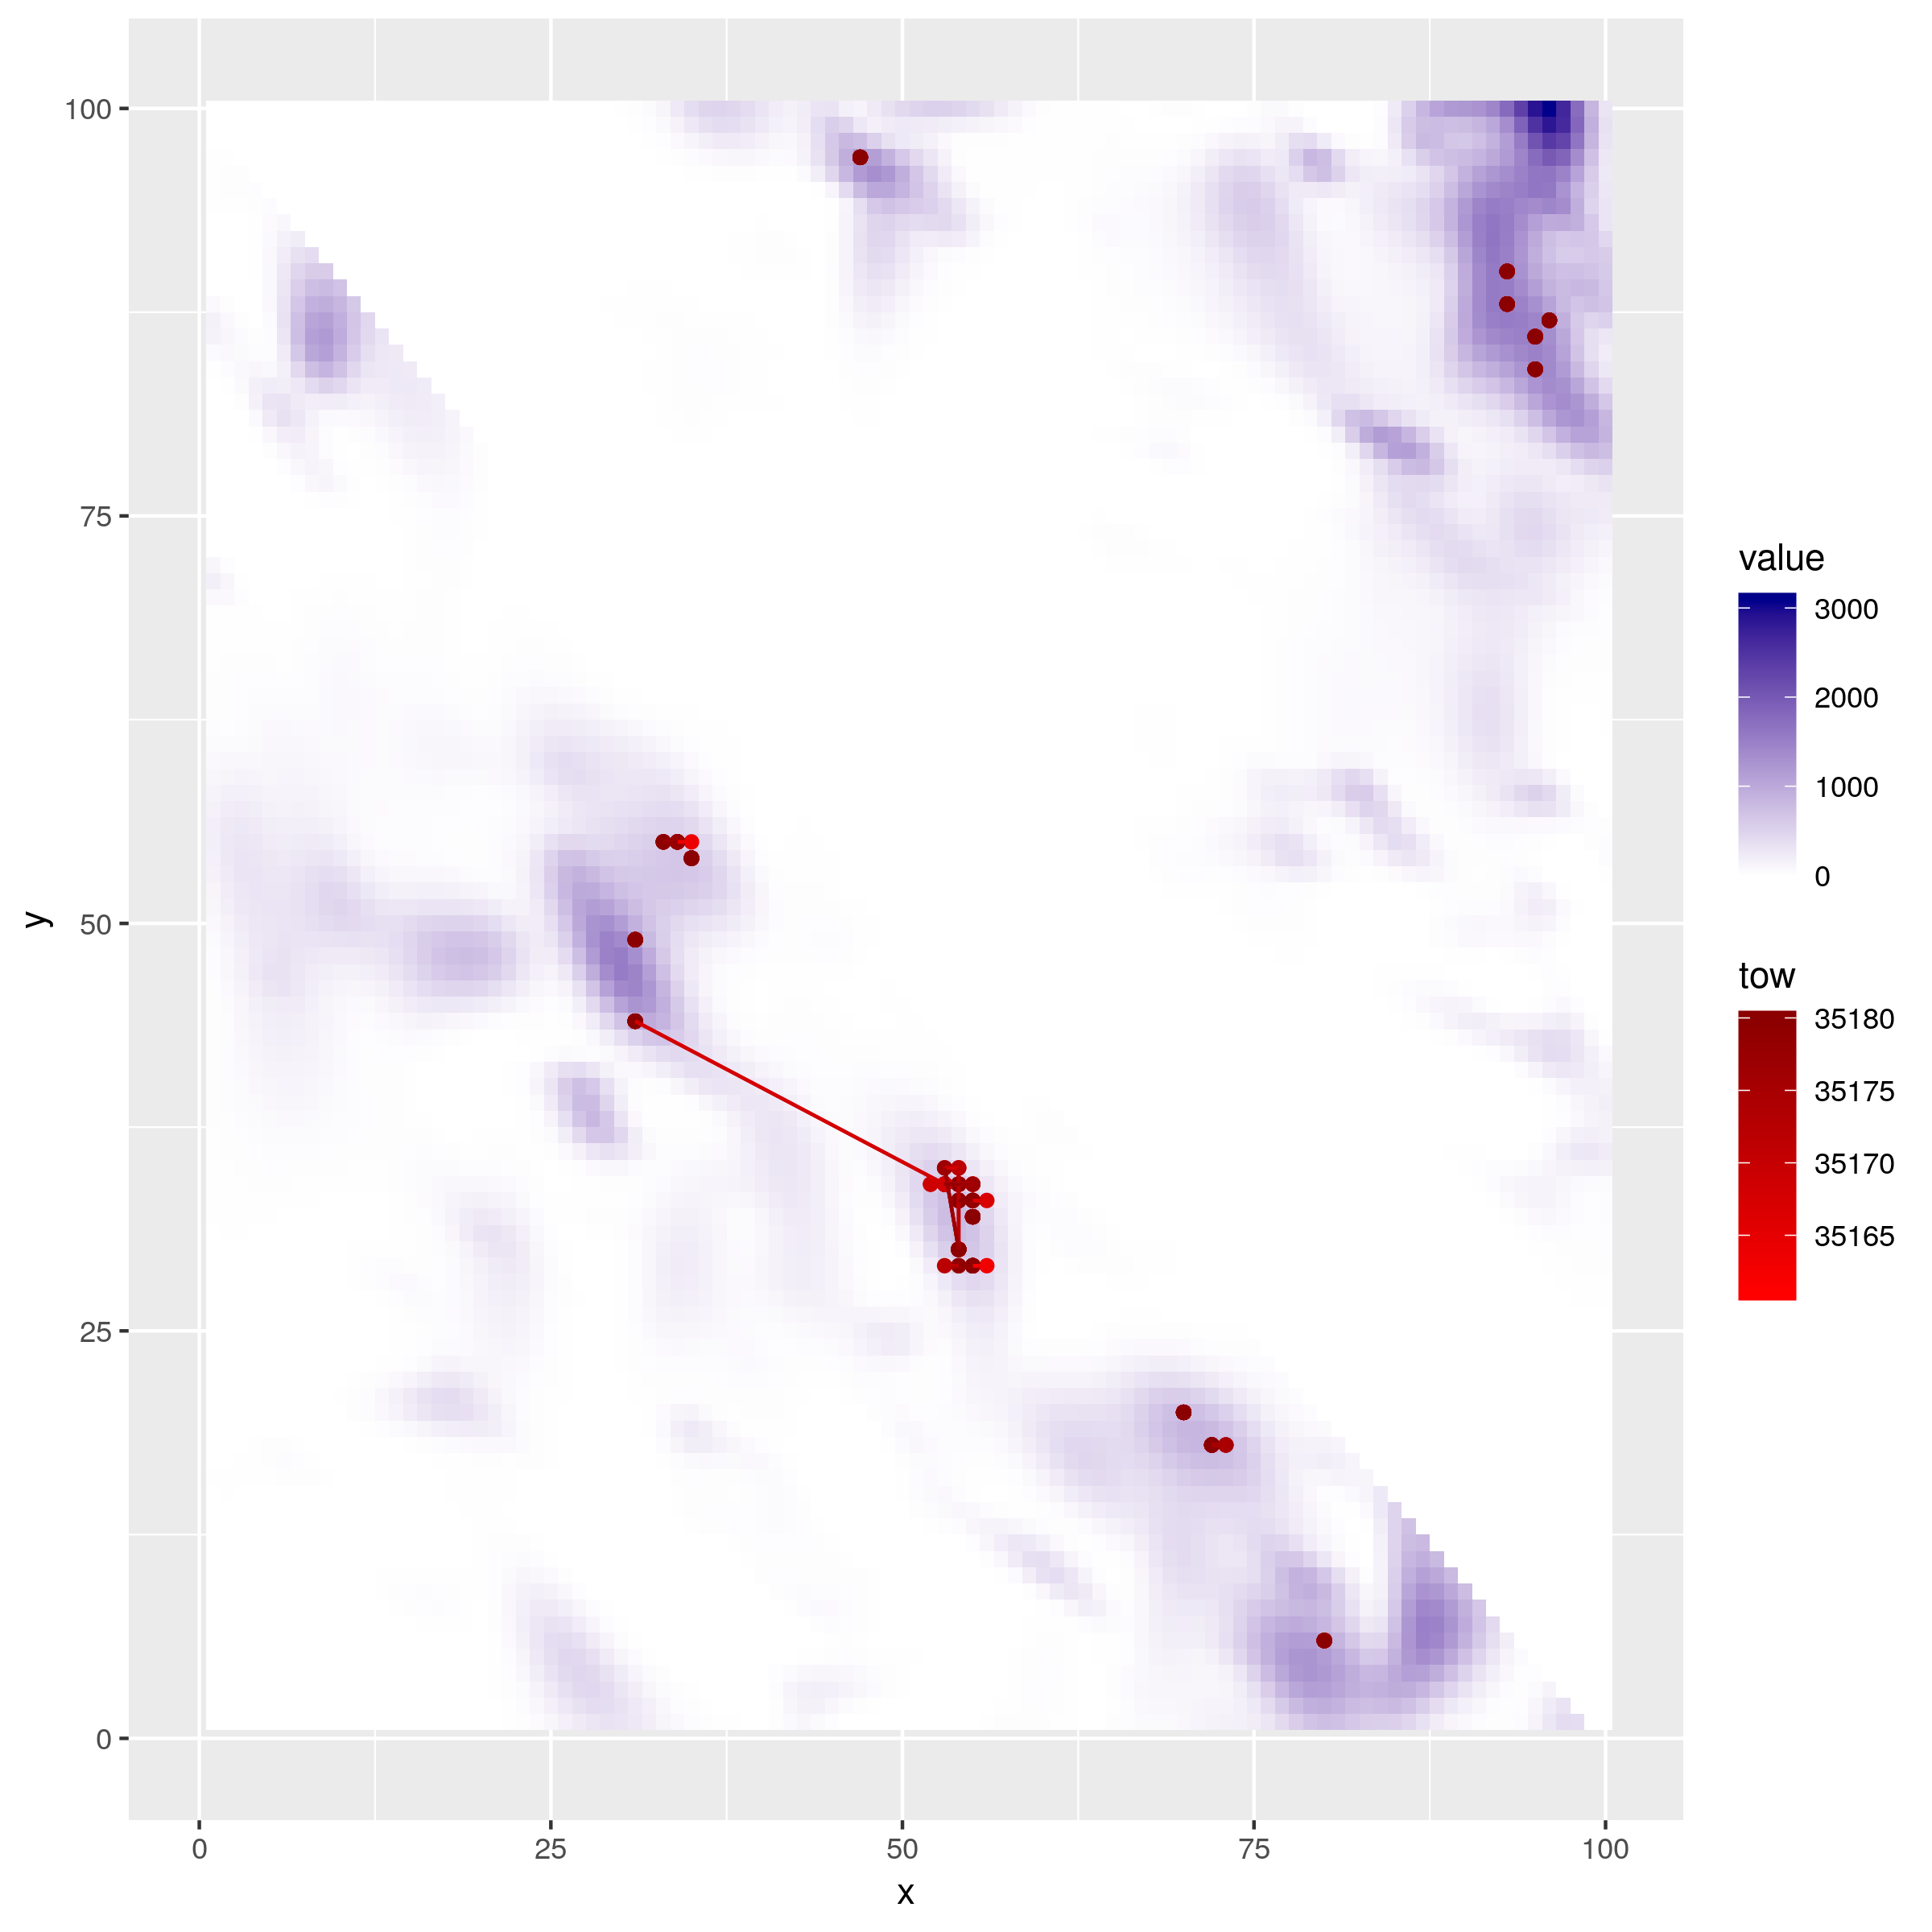
\includegraphics[width = \linewidth]{Plots/vessel_move_value}
	\caption{movement of a single vessel over a few trips overlaid on the
		value field (i.e. sum of the population abundance x catchability x value}
	\label{fig:13}
\end{figure}	

\begin{figure}[!ht]
	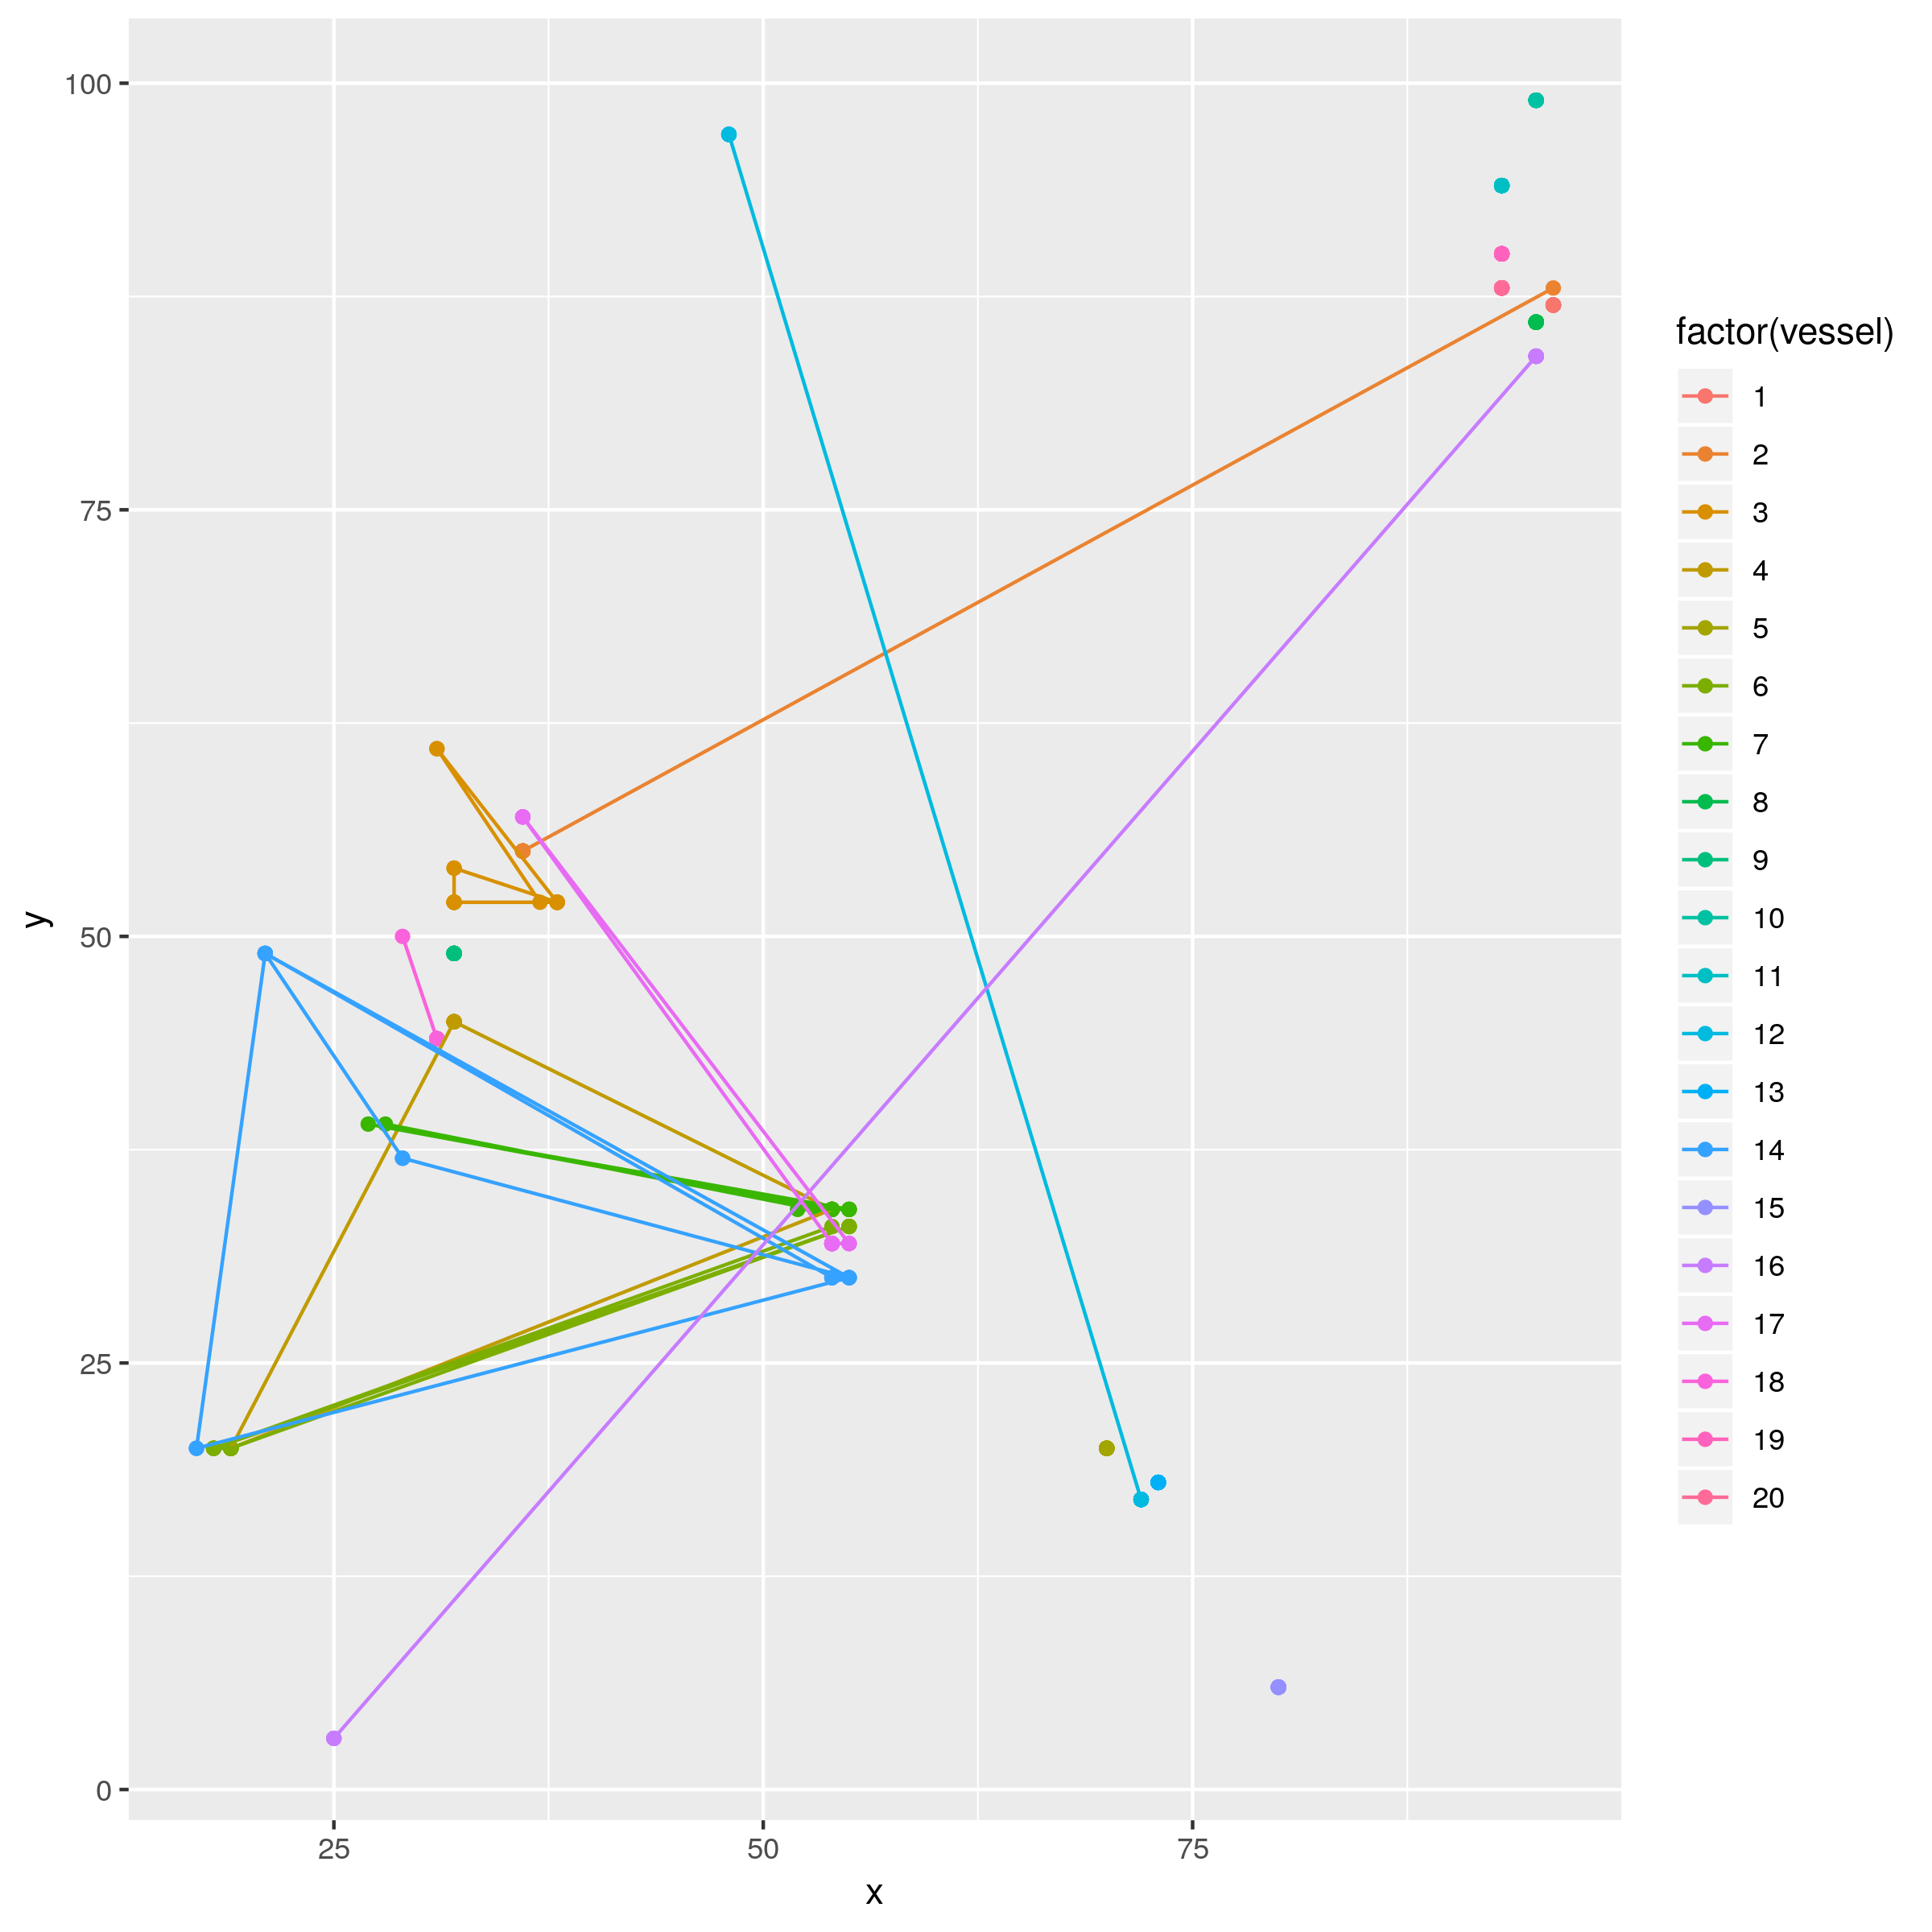
\includegraphics[width = \linewidth]{Plots/fleet_moves}
	\caption{An entire fleets (20 vessels) movement for a single trip}
	\label{fig:14}
\end{figure}	

\begin{figure}[!ht]
	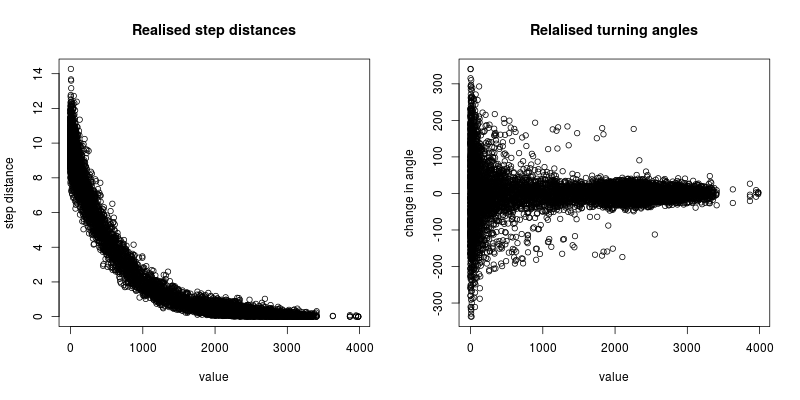
\includegraphics[width = \linewidth]{../tests/plots/step_function}
	\caption{Realised step function - the step function as realised for a
		single fleet. For turning angles, it can be seen that at higher
	values, the turning range is less}
	\label{fig:15}
\end{figure}	



\end{document}

